% vim: set textwidth=78 autoindent:

% \section{Working with Raster Data}\label{label_raster}
\section{Travailler sur des donn\'ees raster}\label{label_raster}
\index{couches raster|(}

% when the revision of a section has been finalized, 
% comment out the following line:
%\updatedisclaimer

% This Section describes how to visualize and set raster layer properties.
% QGIS supports a number of different raster formats. Currently tested formats
% include:\index{raster layers!data formats}
Cette section explique comment visualiser et d\'efinir les propri\'et\'es d'une couche
raster. QGIS g\`ere diff\'erents formats raster. Aujourd'hui les formats test\'es
incluent :\index{couches raster!formats de donn\'ees}
\begin{itemize}
\item Arc/Info Binary Grid
\item Arc/Info ASCII Grid
\item Raster GRASS
\item GeoTIFF
\item JPEG
\item Spatial Data Transfer Standard Grids (avec quelques limitations)
\item DEM ASCII de l'USGS
\item Erdas Imagine
\end{itemize}

% Because the raster implementation in QGIS is based on the GDAL library, other
% raster formats implemented in GDAL are also likely to work - if in doubt try 
% to open a sample and see if it is supported. You find more details about GDAL 
% supported formats in Appendix \ref{appdx_gdal}
% \index{raster layers!GDAL implementation} or at 
% \url{http://www.gdal.org/formats_list.html}. If you want to load GRASS raster 
% data, please refer to Section~\ref{sec:load_grassdata}.
Puisque l'impl\'ementation du raster dans QGIS est bas\'ee sur la biblioth\`eque
GDAL, les autres formats raster impl\'ement\'es dans GDAL fonctionnent aussi
probablement - dans le doute essayez d'ouvrir un fichier test et voyez s'il est
g\'er\'e. Vous trouverez plus d'information sur les formats g\'er\'es par GDAL  en
appendice \ref{appdx_gdal} \index{couches raster!impl\'ementation de GDAL} ou sur
\url{http://www.gdal.org/formats_list.html}. Si vous d\'esirez charger des
donn\'ees raster GRASS, r\'ef\'erez vous \`a la section~\ref{sec:load_grassdata}.

% \subsection{What is raster data?}\label{label_whatsraster}
\subsection{Que sont les donn\'ees raster ?}\label{label_whatsraster}
\index{couches raster !d\'efinition}

% Raster data in GIS are matrices of discrete cells that represent features on,
% above or below the earth's surface. Each cell in the raster grid is the same
% size, and cells are usually rectangular (in QGIS they will always be
% rectangular). Typical raster datasets include remote sensing data such as
% aerial photography or satellite imagery and modelled data such as an elevation
% matrix.
Les donn\'ees raster dans les SIG sont des matrices de cellules discr\`etes qui
repr\'esentent des objets, au dessus ou en dessous de la surface de la terre.
Chaque cellule dans la grille raster est de la m\^eme taille et les cellules sont
g\'en\'eralement rectangulaires (dans QGIS elles seront toujours rectangulaires).
Un jeu de donn\'ees raster typique incluent les donn\'ees des capteurs distants
telles que les photographies a\'eriennes ou les images de satellites et les
donn\'ees mod\'elis\'ees telles que les matrices d'\'el\'evation.

% Unlike vector data, raster data typically do not have an associated database
% record for each cell. They are geocoded by its pixel resolution and the x/y 
% coordinate of a corner pixel of the raster layer. This allows QGIS to
% position the cata correctly in the map canvas.
Contrairement aux donn\'ees vecteurs, les donn\'ees raster n'ont typiquement pas de
base de donn\'ees d'enregistrement associ\'ees. Elles sont g\'eocod\'ees par leur
r\'esolution de pixel et leurs coordonn\'ees x/y du coin du pixel de la couche
raster. Cela permet \`a QGIS de positioner les donn\'ees correctements dans la zone
de la carte.

% QGIS makes use of georeference information inside the raster layer (e.g.
% GeoTiff) or in an appropriate world file to properly display the
% data.\index{raster layers!georeferenced}
QGIS utilise les informations de g\'eor\'ef\'erencement dans les couches raster (par
exemple GeoTiff) ou dans un fichier world appropri\'e pour afficher correctement
les donn\'ees.\index{couches raster!g\'eor\'ef\'erencer}

% \subsection{Loading raster data in QGIS}\label{label_loadraster}
\subsection{Charger des donn\'ees raster dans QGIS}\label{label_loadraster}

% Raster layers are loaded either by clicking on the 
% \toolbtntwo{mActionAddRasterLayer}{Load Raster} icon or by selecting the 
% \mainmenuopt{View}>\dropmenuopttwo{mActionAddRasterLayer}{Add Raster Layer} 
% menu option. More than one layer can be loaded at the same time by holding
% down the \keystroke{Control} or \keystroke{Shift} key and clicking on multiple
% items in the dialog \dialog{Open a GDAL Supported Raster Data
% Source}.\index{raster layers!loading}
Les couches raster sont charg\'ees soit en cliquant sur l'ic\^one
\toolbtntwo{mActionAddRasterLayer}{Charger une couche raster} soit en
s\'electionnant l'option du menu
\mainmenuopt{Couches}>\dropmenuopttwo{mActionAddRasterLayer}{Ajouter une
couche raster}. Plus d'une couche peut \^etre charg\'ee en m\^eme temps en appuyant
sur la touche \keystroke{Control} ou \keystroke{Shift} et en cliquant sur de
plusieurs couches dans la bo\^ite de dialogue \dialog{Ouvrez des sources de
donn\'ees taster g\'er\'es par GDAL}.\index{couches raster!charger}

% Once a raster layer is loaded in the map legend you can click on the layer
% name with the right mouse button to select and activate layer specific
% features or to open a dialog to set raster properties for the layer.
Une fois la couche raster charg\'ee dans la l\'egende de la carte vous pouvez
cliquer sur le nom de la couche avec le bouton droit de la souris pour
s\'electionner et activer des param\`etres sp\'ecifiques \`a la couche ou pour ouvrir
une bo\^ite de dialogue pour d\'efinir des propri\'et\'es du raster pour la couche.

% \minisec{Right mouse button menu for raster layers}
\minisec{Menu du bouton droit de la souris pour les couches raster}

\begin{itemize}
% \item \dropmenuopt{Zoom to layer extent}
% \item \dropmenuopt{Zoom to best scale (100\%)}
% \item \dropmenuopt{Show in overview}
% \item \dropmenuopt{Remove}
% \item \dropmenuopt{Properties}
% \item \dropmenuopt{Rename}
% \item \dropmenuopt{Add Group}
% \item \dropmenuopt{Expand all}
% \item \dropmenuopt{Collapse all}
% \item \dropmenuopt{Show file groups}
\item \dropmenuopt{Zoom sur l'\'etendue de la couche}
\item \dropmenuopt{Zoom \`a la meilleur \'echelle (100\%)}
\item \dropmenuopt{L'affiche dans l'aper\c{c}u}
\item \dropmenuopt{Supprime}
\item \dropmenuopt{Propri\'et\'es}
\item \dropmenuopt{Renomer}
\item \dropmenuopt{Ajouter un groupe}
\item \dropmenuopt{Tout \'et\'endre }
\item \dropmenuopt{Tout diminuer}
\item \dropmenuopt{Afficher les groupes du fichier}
\end{itemize}

% \subsection{Raster Properties Dialog}\label{label_rasterprop}
\subsection{bo\^ite de dialogue de propri\'et\'es des Raster}\label{label_rasterprop}

% To view and set the properties for a raster layer, double click 
% on the layer name in the map legend or right click on the layer name and
% choose \dropmenuopt{Properties} from the context menu:\index{raster
% layers!context menu} Figure \ref{fig:raster_properties} shows the
% \dialog{Raster Layer Properties} dialog. There are several tabs on the
% dialog: 
Pour voir et d\'efinir les propri\'et\'es d'une couche raster, double-cliquez sur le
nom de la couche dan la l\'egende de la carte ou cliquez droit sur le nom de
lacouche et choisissez \dropmenuopt{Propri\'et\'es} du menu
contextuel:\index{couche raster!menu contextuel}  Figure
\ref{fig:raster_properties} montre la bo\^ite de dialogue \dialog{Propri\'et\'es
de la couche raster}. Il y a plusieurs onglets dans cette fen\^etre :

\begin{itemize}
%  \item \tab{Symbology}
%  \item \tab{Transparency}
%  \item \tab{Colormap}
%  \item \tab{General}
%  \item \tab{Metadata}
%  \item \tab{Pyramids}
%  \item \tab{Histogram}
 \item \tab{S\'emiologie}
 \item \tab{Transparence}
 \item \tab{Carte de couleur}
 \item \tab{G\'en\'eral}
 \item \tab{M\'eta-donn\'ees}
 \item \tab{Pyramides}
 \item \tab{Histograme}
\end{itemize}

\begin{figure}[h]
  \begin{center}
%    \caption{Raster Layers Properties Dialog
% \nixcaption}\label{fig:raster_properties}\smallskip
   \caption{bo\^ite de dialogue des propri\'et\'es des couches raster
\nixcaption}\label{fig:raster_properties}\smallskip
   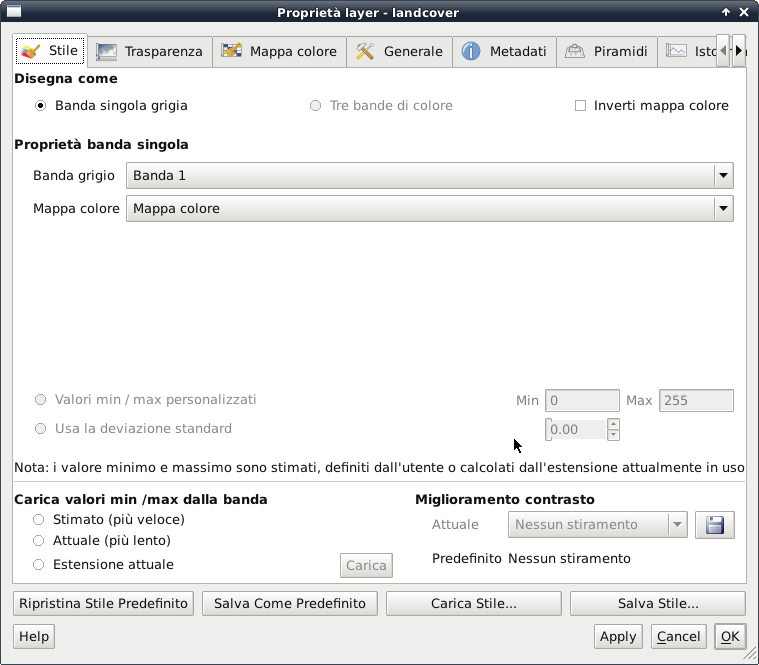
\includegraphics[clip=true, width=14cm]{rasterPropertiesDialog}
\end{center}
\end{figure}

\subsubsection{Onlget s\'emiologie}\label{label_sombology}

% QGIS can render raster layers in two different ways :\index{raster
% layers!supported channels}
QGIS peut afficher des couches raster de deux mani\`eres diff\'erentes
:\index{couches layers!canaux g\'er\'es}

\begin{itemize}
% \item Single band - one band of the image will be rendered as gray or in 
% pseudocolors.
\item Bande simple - une bande de l'image sera affich\'ee en nuance de gris ou en
pseudocouleurs.
% \item Three band color - three bands from the image will be rendered, each 
% band representing the red, green or blue component that will be used to
% create a color image.
\item Trois bandes de couleurs - trois bandes de l'image seront affich\'ees,
chaque bande repr\'esentant le composant rouge, vert ou bleu qui sera utilis\'e
pour cr\'eer une image de couleur.
\end{itemize}

% Within both rendertypes you can invert the color output using the 
% \checkbox{Invert color map} checkbox.
Pour les deux types de rendu vous pouvez inverser la sortie couleur en
utilisant la case \`a cocher \checkbox{Inverser la carte de couleur}

% \minisec{Single Band Rendering}
\minisec{Rendu des bandes simples}

% This selection offers you two possibilites to choose. At first you can
% select which band you like to use for rendering (if the dataset has more than 
% one band).
Ce choix vous permet deux possibilit\'es : vous pouvez d'abord s\'electionner
quelle bande vous voulez utiliser pour le rendu (si le jeu de donn\'ees a plus
d'une bande).

% The second option offers a selection of available colortables for rendering.
La seconde option vous offre une s\'election des tables de couleurs disponibles
pour le rendu.

% The following settings are available through the dropdownbox
% \selectstring{color map}{Grayscale}, where grayscale is the default setting.
Les param\`etres suivants sont disponibles \`a travers la liste d\'eroulante
\selectstring{carte de couleur}{Niveau de gris}, o\`u niveau de gris est le 
param\`etre par d\'efaut.

% Also available are
Sont aussi disponible :
\begin{itemize}
% \item Pseudocolor
\item Pseudo-couleur
% \item Freak Out
\item Pseudo-couleur psych\'ed\'elique
% \item Colormap
\item Couleurs index\'ees
\end{itemize}

% When selecting the entry \selectstring{color map}{Colormap}, the tab
% \tab{Colormap} becomes available. See more on that at chapter
% \ref{label_colormaptab}.
Quand vous s\'electionnez \selectstring{couleurs index\'ees}{Colormap}, l'onglet
\tab{Couleurs index\'ees} est disponible. Plus d'informations dans le chapitre
\ref{label_colormaptab}.

% QGIS can restrict the data displayed to only show cells whose values are
% within a given number of standard deviations of the mean for the
% layer.\index{raster layers!standard deviation} This is useful when you have
% one or two cells with abnormally high values in a raster grid that are having
% a negative impact on the rendering of the raster. This option is only
% available for pseudocolor images.
QGIS peut restreindre les donn\'ees affich\'ees pour afficher seulement les
cellules dont la valeur sont dans un nombre donn\'e de d\'eviations standards de
la moyenne pour la couche.\index{couches raster!d\'eviation standard} Cela est
utile quand vous avez une ou deux cellules avec des valeurs anormalement hautes
dans une grille raster qui ont un impact n\'egatif sur le rendu du raster. Cette
option est seulement disponible pour les images en pseudo-couleur.

% \minisec{Three band color}
\minisec{Couleur \`a trois bandes}

% This selection offers you a wide range of options to modify the appereance
% of your rasterlayer. For example you could switch color-bands from the
% standard RGB-order to something else.
Cette s\'election vous offre un large choix d'options pour modifier l'apparence
de votre couche raster. Par exemple, vous pouvez passer les bandes de couleurs
d'un ordre standard RVB \`a un autre.

% Also scaling of colors are available.
L'\'echantillonage des couleurs est \'egalement disponible.

% \begin{Tip}\caption{\textsc{Viewing a Single Band of a Multiband Raster}}
\begin{Tip}\caption{\textsc{Visualiser une seule bande d'un raster multibande}}
% \qgistip{If you want to view a single band (for example Red) of a multiband
% image, you might think you would set the Green and Blue bands to ``Not
% Set''. But this is not the correct way. To display the Red band, 
% set the image type to grayscale, then select Red as the band to use for Gray.
\qgistip{Si vous d\'esirez visualiser une seule bande (par exemple la bande rouge)
d'une image multibande, vous pouvez penser que vous pourriez d\'efinir les bandes
Vertes et Bleue \`a ``Non d\'efinie''. Mais ce n'est pas la mani\`ere correcte. Pour
afficher la bande Rouge d\'efinissez le type d'image \`a nuance de gris, puis
s\'electionnez Rouge comme bande \`a utiliser pour le Gris.
}
\end{Tip} 

% \subsubsection{Transparency Tab} \label{rastertab:transparency}
\subsubsection{Onglet transparence} \label{rastertab:transparency}

% QGIS has the ability to display each raster layer at varying transparency
% levels.\index{raster layers!transparency} Use the transparency slider to
% indicate to what extent the underlying layers (if any) should be visible
% though the current raster layer. This is very useful, if you like to overlay
% more than one rasterlayer, e.g. a shaded relief-map overlayed by a classified
% rastermap. This will make the look of the map more three dimensional.
QGIS a la possibilit\'e d'afficher chaque raster \`a des niveaux de transparence
diff\'erents.\index{couches raster!transparence} Utiliser la barre coulissante de
transparence pour indiquer \`a quel niveau de transparence les couches sous-jacentes
(s'il y en a) pourront \^etre visible \`a travers cette couche raster. Cela est
tr\`es utile, si vous d\'esirez superposer plus d'une couche raster, par exemple
une carte des reliefs ombr\'es superpos\'e par une carte raster classifi\'ee. Cela
rendra la carte encore plus proche de la 3e dimension.

% Additionally you can enter a rastervalue, which should be treated as
% {\em NODATA}.
De plus, vous pouvez entrer une valeur raster qui pourra \^etre trait\'e comme {\em
NODATA}

% An even more flexible way to customize the transparency can be done in the
% \guiheading{Custom transparency options} section.
% The transparency of every pixel can be set in this tab.
Un moyen encore plus flexible pour personnaliser la transparence est possible
dans la section \guiheading{Options de transparence personnalis\'ee}.
La transparence de chaque pixel peut \^etre d\'efinie dans cet onglet.

% As an example we want to set the water of our example rasterfile
% \filename{landcover.tif} to a transparency of 20\%. The following steps
% are neccessary:
Par exemple, nous voulons d\'efinir l'eau de notre fichier raster d'exemple
\filename{landcover.tif} \`a une transparence de 20 \%. Les \'etapes suivantes sont
n\'ecessaire :
\begin{enumerate}
%  \item  Load the rasterfile \filename{landcover}
\item Chargez le fichier raster \filename{landcover}
%  \item Open the \dialog{properties} dialog by double-clicking on the
%  rasterfile-name in the legend or by right-clicking and choosing
%  \dropmenuopt{Properties} from the popup meun.
 \item Ouvrez la bo\^ite de dialogue \dialog{propri\'et\'ees} en double-cliquant sur
le nom du raster dans la l\'egende ou avec un clic droit et en choisissant
\dropmenuopt{Propri\'et\'ees} du menu contextuel.
%  \item select the \tab{Transparency} tab
 \item S\'electionnez l'onglet \tab{Transparence}.
% \item \label{enum:add} Click the \toolbtntwo{mActionNewAttribute}{Add values
% manually} button. A new row will appear in the pixel-list.
  \item \label{enum:add} Cliquez sur le bouton
\toolbtntwo{mActionNewAttribute}{Ajouter des valeurs manuellement}. Une
nouvelle ligne apparait dans la liste des pixels.
%  \item \label{enum:transp} enter the the raster-value (we use 0 here) and
% adjust the  transparency to 20\%
 \item \label{enum:transp} Entrez la valeur du raster (nous utilisons 0 ici)
et ajustez la transparence \`a 20 \%.
%  \item press the \button{Apply} button and have a look at the map
 \item Pressez le bouton \button{Appliquer} et regardez la carte.
\end{enumerate}

% You can repeat the steps \ref{enum:add} and \ref{enum:transp} to adjust
% more values with custom transparency.
Vous pouvez r\'ep\'eter les \'etapes \ref{enum:add} et \ref{enum:transp} pour ajuster
d'autres valeurs avec une transparence personnalis\'ee. 

% As you can see this is quite easy set custom transparency, but it can be
% quite a lot of work. Therefor you can use the button
% \toolbtntwo{mActionFileSave}{Export to file} to save your transparency-list to
% a file. The button \toolbtntwo{mActionAddRasterLayer}{Import from file} loads
% your transparency-settings and applies them to the current rasterlayer.
Comme vous pouvez le voir il est assez facile de d\'efinir une transparence
personnalis\'ee, mais cela peut prendre un peu de temp. Par cons\'equent vous
pouvez utiliser le bouton \toolbtntwo{mActionFileSave}{Exporter dans un
fichier} pour sauver vos param\`etres  de transparence dans un fichier. Le
bouton \toolbtntwo{mActionAddRasterLayer}{Importer \`a partir d'un fichier} 
charge vos param\`etres de transparence et les applique \`a la couche raster actuel.

% \subsubsection{Colormap} \label{label_colormaptab}
 \subsubsection{Carte de couleur} \label{label_colormaptab}
% FIXME: Write me

% The \tab{Colormap} tab is only available, when you have selected a
% single-band-rendering within the tab \tab{Symbology} (see chapt.
% \ref{label_sombology}).
L'onglet \tab{Colormap} est seulement disponible quand vous avez s\'electionn\'e un
rendu \`a une seule bande dans l'onglet  \tab{S\'emiologie} (voir chapitre
\ref{label_sombology}).

% Three ways of color interpolation are available:
Trois mani\`eres de faire une interpolation de couleur sont disponibles :
\begin{itemize}
% \item Discrete
\item discr\`ete ;
% \item Linear
\item li\'enaire ;
% \item Exact
\item exacte.
\end{itemize}

% The button \button{Add Entry} adds a color to the individual color-table.
% Double-Clicking on the value-column lets you inserting a specific value.
% Double clicking on the color-column opens the dialog \dialog{Select
% color} where you can select a color to apply on that value.
Le bouton \button{Ajouter une entr\'ee} ajoute une couleur \`a la table de couleur
individuelle. Double-cliquez sur la colonne valeur vous permet d'ins\'erer une
valeur sp\'ecifique. Double-cliquez sur la colonne couleur ouvre une bo\^ite de
dialogue \dialog{S\'electionner une couleur}  o\`u vous pouvez s\'electionner une
couleur \`a appliquer sur cette valeur.

% Alternativly you can click on the button \toolbtntwo{mActionNewAttribute}{Load
% colormap from Band} , which tries to load the table from the band (if it has
% any).
Alternativement, vous pouvez cliquer sur le bouton
\toolbtntwo{mActionNewAttribute}{charger une carte de couleur \`a partir de
bande}  qui tente de charger la table \`a partir d'une bande (si celle-ci en a
une).

% The block \guiheading{Generate new color map} allows you to create newly
% categorized colormaps. You only need to select the \selectnumber{number of
% classes}{15} you need and press the button \button{Classify}. Currently
% only one \selectstring{Classification mode}{Equal Interval} is
% supported\index{raster layer!classify}.
Le bloc \guiheading{G\'en\`erer une nouvelle carte de couleurs} vous permet de
cr\'eer de nouvelles cartes de couleurs par cat\'egorie. Vosu avez seulement besoin
de s\'electionner le \selectnumber{nombre de classes}{15} dont vous avez besoin
et d'appuyez sur le bouton \button{Classifier}. Actuellement seule un 
\selectstring{mode de classification}{intervals \'egaux} est g\'er\'e\index{couches
raster!classifier}.

% \subsubsection{General Tab}\label{label_generaltab}
\subsubsection{Onglet g\'en\'eral}\label{label_generaltab}

% The \tab{General} tab displays basic information about the selected raster,
% including the layer source and  display name in the legend (which can be
% modified). This tab also shows a thumbnail of the layer, its legend symbol,
% and the palette.\index{raster layers!properties}
L'onglet \tab{G\'en\'eral} affiche des informations basiques sur le raster
s\'electionn\'e, incluant la source de la couche et le nom affich\'e dans la l\'egende
(qui peut \^etre modifi\'e). Cet onglet montre aussi un aper\c{c}u de la couche, le
symbol de la l\'egende, et la palette.\index{couches raster!propri\'et\'es}

% Additionally scale-dependent visability can be set in this tab. You need to
% check the checkbox and set an appropriate scale where your data will be
% displayed in the map canvas.
De plus la visibilit\'e en fonction de l'\'echelle peut \^etre d\'efinie dans cet
onglet. Vous devez activer la case \`a cocher et d\'efinir une \'echelle appropri\'ee \`a
laquelle vos donn\'ees seront affich\'ees dans la fen\^etre de la carte.

% Also the spatial reference system is printed here as a PROJ.4-string. This can
% be modified by hitting the \button{Change} button.
Le syst\`eme de r\'ef\'erence spatial est \'egalement affich\'e ici comme cha\^ine PROJ.4.
Cela peut \^etre modifi\'e en cliquant sur le bouton \button{Changer}.

% \subsubsection{Metadata Tab}\label{label_metatab}
\subsubsection{Onglet m\'eta-donn\'ees}\label{label_metatab}

% The \tab{Metadata} tab displays a wealth of information about the raster
% layer, including statistics about each band in the current raster layer.
% Statistics are gathered on a 'need to know' basis, so it may well be that a
% given layers statistics have not yet been collected.\index{raster
% layers!metadata}
L'onglet \tab{M\'eta-donn\'ees} affiche toute la richesse d'information sur la
couche raster, dont les statistiques sur chaque bande dans la couche raster
actuelle. Les statistiques sont recueillies sur l'id\'ee de la 'n\'ecessit\'e de
savoir', de sorte qu'il est possible qu'une couche n'ait pas de
statistique collect\'ee.\index{couches raster!m\'eta-donn\'ees} 

% This tab is mainly for information. You cannot change any values printed
% inside this tab. To update the statistics you need to change to tab
% \tab{Histogram} and press the button \button{Refresh} on the bottom right,
% see ch. \ref{label_histogram}.
Cet onglet est principalement pour informations. Vous ne pouvez pas modifier
les valeurs qui y sont affich\'ees. Pour mettre \`a jour les statistiques vous
devez aller dans l'onglet \tab{Histogramme} et pressez le bouton
\button{Rafraichir} en bas \`a droite, voir chapitre \ref{label_histogram}.

% \subsubsection{Pyramids Tab}\label{raster_pyramids}
\subsubsection{Onglet pyramides}\label{raster_pyramids}

% Large resolution raster layers can slow navigation in QGIS. By creating lower
% resolution copies of the data (pyramids), performance can be considerably
% improved as QGIS selects the most suitable resolution to use depending on the
% level of zoom.
Les couches raster \`a haute r\'esolution peuvent ralentir la navigation dans QGIS.
En cr\'eant des copies de plus basse r\'esolution des donn\'ees (pyramides), les
performances peuvent \^etre consid\'erablement am\'elior\'ees puisque QGIS s\'electionne
la r\'esolution la plus pertinente \`a utiliser en fonction du niveau de zoom.

% \index{raster layers!pyramids}
\index{couches raster!pyramides}
% \index{raster layers!resolution pyramids}
\index{couches raster!r\'esolution des pyramides}

% You must have write access in the directory where the original data is stored
% to build pyramids. \\
Vous devez avoir acc\`es en \'ecriture dans le r\'epertoire o\`u les donn\'ees
originelles sont stock\'ees pour construire les pyramides. \\
% Several resampling methods can be used to calculate the pyramides:
Plusieurs m\'ethodes de re\'echantillonage peuvent \^etre utilis\'ees pour calculer les
pyramides :
\begin{itemize}
% \item Average
\item moyen
% \item Nearest Neighbour
\item plus proche voisin ;
\end{itemize}

% When checking the checkbox \checkbox{Build pyramids internally if
% possible} QGIS tries to build pyramids internally.
Quand la case \checkbox{construire les pyramides en interne si possible} est
coch\'ee, QGIS tente de construire les pyramides en interne.

% Please note that building pyramids may alter the original data file and once
% created they cannot be removed. If you wish to preserve a 'non-pyramided'
% version of your raster, make a backup copy prior to building pyramids.
S'il vous plait notez que construire des pyramides peut alt\'erer les fichiers
donn\'ees originaux et une fois cr\'e\'e ils ne peuvent plus \^etre supprim\'e. Si vous
d\'esirez pr\'eserver une version 'sans pyramide' de vos raster, r\'ealisez une copie
de sauvegarde avant de les construire.

% \subsubsection{Histogram Tab}\label{label_histogram}
\subsubsection{Onglet histograme}\label{label_histogram}

% The \tab{Histogram} tab allows you to view the distribution\index{raster
% layers!histogram} of the bands or colors in your raster. You must first
% generate the raster statistics by clicking the \button{Refresh} button. You
% can choose which bands to display by selecting them in the list box at the
% bottom left of the tab. Two different chart types are allowed: 
L'onglet \tab{Histogramme}  vous permet de visualiser la distribution
\index{couches raster!histogramme} des bandes ou des couleurs dans votre
raster. Vous devez d'abord g\'en\'erer les statistiques du raster en cliquant le
bouton \button{Rafraichir}. Vous pouvez choisir quelles bandes \`a afficher en
les s\'electionnant dans la liste d\'eroulante en bas \`a gauche de l'onglet. Deux
types de graphiques diff\'erents sont permis :

\begin{itemize}
% \item Bar chart
\item graphique en barre ;
% \item Line graph
\item graphique lin\'eaire ;
\end{itemize}

% You can define the number of chart columns to use and decide wether you want 
% to \checkbox{Allow approximation} or display \checkbox{out of range} values 
% Once you view the histogram, you'll notice that the band statistics have been
% populated on the \tab{metadata} tab.\index{raster layers!metadata)}
Vous pouvez d\'efinir le nombre de colonnes du graphique \`a utiliser et d\'ecider si
vous voulez \checkbox{Permettre l'approximation} ou afficher les valeurs
\checkbox{En dehors du domaine}. Une fois que vous avez vu l'histogramme, vous
remarquerez que les statistiques des bandes ont \'et\'e remplies dans l'onglet
\tab{m\'eta-donn\'ees}.\index{couches raster!m\'eta-donn\'ees}

% \begin{Tip}\caption{\textsc{Gathering Raster Statistics}}
\begin{Tip}\caption{\textsc{Regroupement des statistiques raster}}
% \qgistip{To gather statistics for a layer, select pseudocolor rendering and
% click the \button{Apply} button. Gathering statistics for a layer can be time
% consuming. Please be patient while QGIS examines your
% data!\index{raster layers!statistics}
\qgistip{Rassembler des statistiques pour une couche, s\'electionnez un rendu en
pseudo-couleur et cliquez sur le bouton \button{Appliquer}. Regrouper des
statistiques pour une couche peut prendre du temp. Soyez patient pendant que
QGIS examine  vos donn\'ees !\index{couches raster!statistiques}
}
\end{Tip}
